\newpage
\section{Проектирование программных средств и их частей}

\subsection{Описание требований}

\subparagraph{Требуемая функциональность программы:}\hspace{0pt}

\begin{itemize}
  \item \textbf{регистрация} - пользователь может зарегистрироваться введя его имя, электронную почту, логин и пароль;
  \item \textbf{авторизация} - полльзоватль может авторизоваться введя логин и пароль;
  \item \textbf{просмотр задач за год} - есть 12 месяцев и рядом с днем два кружка (1 - есть невыполненые задачи, 2 - есть выполненые задача);
  \item \textbf{просмотр задач за месяц} - есть прямоугольник из 42 двух дней (7x6, чтобы поместился любой месяц);
  \item \textbf{просмотр задач на день} - список;
  \item \textbf{просмотр задач по часам} - прямоугольники показывающие продолжительность задания по времени.
\end{itemize}

\subparagraph{Желаемые дополнительные функции:}\hspace{0pt}

\begin{itemize}
  \item \textbf{подтвержнение почты при регистрации} - на почту будет приходить код, который нужно будет ввести на сайте,
  чтобы можно было авторизоваться, а если же пользователь вышел с сайта,
  то перейдя по ссылке можно было подтвердить аккаунт;
  \item \textbf{возможность восстановления пароля} - на почту будет приходить сообщение с ссылкой,
  перейдя по которой можно будет ввести новый пароль;
  \item \textbf{возможность создания мероприятий из любых страниц} - на каждой странице есть особая форма создания мероприятия
  (на год, месяц и день).
\end{itemize}

\subparagraph{Требуемые технические требования:}\hspace{0pt}

\begin{itemize}
  \item \textbf{проведение миграций БД} - разобраться с какой-нибудь ORM, которая может создавать модельки таблицы,
  а так как модельки изменяются, то научиться делать файлы с временой меткой, содержащие изменение модели таблицы.
  \item \textbf{ограниченная авторизация} - при авторизации отсылать клиенту access и refresh токены
  (access токен с временем жизни 15 минут и refresh токен c временем жизни 2 дня,
  который может запросить новый access токен);
  \item \textbf{автоматическия сборка образов из Dockerfile'ов и выгрузка на DockerHub} - в репозитории есть защищенная ветка dev,
  в которую нельзя делать изменения, так как все делается через Pull Request'ы, которая при залитии обновлений из Pull Request'а
  запустит GitHub action, который запустит задача по сборке образа из Dockerfile и по окончанию загрузит на DockerHub.
\end{itemize}

\newpage
\subsection{Варианты использования программы в виде диаграмм прецедентов (Use Case Diagram)}

Первичное описание прецедентов для сотрудника изображено на~рис.~\ref{fig:UseCaseDiagram}.

\begin{figure}[!ph]
  \centering

  \includegraphics[width=18cm]
  {../design/UML/export/UseCaseDiagram-Page-1.pdf}

  \caption{Первичное описание прецедентов (UseCase Diagram)}
  \label{fig:UseCaseDiagram}
\end{figure}


% = = = = = = = = = = = = = = = =
\subparagraph{\underline{Прецендент «Регистрация»}} \hspace{0pt}

\textit{Назначение}: создание нового пользователя.

\textit{Исполнители}: пользователь, браузер.

\textit{Предусловие}: находимся на странице регистрации.

\textit{Основной поток событий}: создали пользователя.

\textit{Альтернативный поток событий}: сервер отошлет ответ, который сообщит почему не зарегистрировался.
% = = = = = = = = = = = = = = = =


% = = = = = = = = = = = = = = = =
\subparagraph{\underline{Прецендент «Авторизация»}} \hspace{0pt}

\textit{Назначение}: проверка логина и пароля.

\textit{Исполнители}: пользователь, браузер.

\textit{Предусловие}: находимся на странице авторизации.

\textit{Основной поток событий}: получили access и refresh токены.

\textit{Альтернативный поток событий}: сервер отошлет ответ, который сообщит почему не авторизовался.
% = = = = = = = = = = = = = = = =


% = = = = = = = = = = = = = = = =
\newpage
\subparagraph{\underline{Прецендент <<Создание мероприятия>>}} \hspace{0pt}

\textit{Назначение}: создание мероприятия в календаре пользователя.

\textit{Исполнители}: пользователь, браузер.

\textit{Предусловие}: access токен не просрочен и не подделынный.

\textit{Основной поток событий}: в базе данных добавилось мероприятие.

\textit{Альтернативный поток событий}: сервер отошлет ответ, который сообщит почему не создалось мероприятие.
% = = = = = = = = = = = = = = = =


% = = = = = = = = = = = = = = = =
\subparagraph{\underline{Прецендент <<Просмотр мероприятий>>}} \hspace{0pt}

\textit{Назначение}: получить массив всех мероприятий.

\textit{Исполнители}: пользователь, браузер.

\textit{Предусловие}: access токен не просрочен и не подделынный.

\textit{Основной поток событий}: получили массив мероприятий.

\textit{Альтернативный поток событий}: сервер отошлет ответ, который сообщит почему не получили массив мероприятий.
% = = = = = = = = = = = = = = = =


% = = = = = = = = = = = = = = = =
\subparagraph{\underline{Прецендент <<Просмотр мероприятия по id>>}} \hspace{0pt}

\textit{Назначение}: получить данные мероприятия по id.

\textit{Исполнители}: пользователь, браузер.

\textit{Предусловие}: access токен не просрочен и не подделынный.

\textit{Основной поток событий}: получили данные мероприятия по id.

\textit{Альтернативный поток событий}: сервер отошлет ответ, который сообщит почему не получили данные мероприятия по id.
% = = = = = = = = = = = = = = = =


% = = = = = = = = = = = = = = = =
\subparagraph{\underline{Прецендент <<Изменение мероприятия по id>>}} \hspace{0pt}

\textit{Назначение}: изменить данные мероприятия по id.

\textit{Исполнители}: пользователь, браузер.

\textit{Предусловие}: access токен не просрочен и не подделынный.

\textit{Основной поток событий}: обновляем мероприятие в базе данных по id.

\textit{Альтернативный поток событий}: сервер отошлет ответ, который сообщит почему не изменили данные мероприятия по id.
% = = = = = = = = = = = = = = = =


% = = = = = = = = = = = = = = = =
\subparagraph{\underline{Прецендент <<Удаление мероприятия по id>>}} \hspace{0pt}

\textit{Назначение}: удаляем мероприятие по id.

\textit{Исполнители}: пользователь, браузер.

\textit{Предусловие}: access токен не просрочен и не подделынный.

\textit{Основной поток событий}: удаляем мероприятие в базе данных по id.

\textit{Альтернативный поток событий}: сервер отошлет ответ, который сообщит почему не удалили мероприятие по id.
% = = = = = = = = = = = = = = = =


% = = = = = = = = = = = = = = = =
\newpage
\subsection{Первичное описание моделей}

% = = = = = = = = = = = = = = = =
\subparagraph{Пользователи} \hspace{0pt}

Модель таблицы для хранения пользователей со следующими атрибутами:
\begin{itemize}
  \item id - идентификатор пользователя
  \item Name - как обращаться к пользователю
  \item Email - электронная почта пользователя
  \item Login - логин пользователя
  \item HashPassword - захэшированный пароль пользователя
\end{itemize}
% = = = = = = = = = = = = = = = =

% = = = = = = = = = = = = = = = =
\subparagraph{Мероприятие} \hspace{0pt}

Модель таблицы для хранения мероприятий со следующими атрибутами:
\begin{itemize}
  \item id - идентификатор мероприятия
  \item Name - Наименование мероприятия
  \item Description - описание мероприятия
  \item IsCompleted - выполнено ли задание
  \item StartDate - начало мероприятия
  \item EndDate - конец мероприятия
\end{itemize}
% = = = = = = = = = = = = = = = =

% = = = = = = = = = = = = = = = =
\subparagraph{Access токены} \hspace{0pt}

Модель таблицы для хранения токенов со следующими атрибутами:
\begin{itemize}
  \item id - идентификатор
  \item UserId - идентификатор пользователя
  \item AccessToken - токен
\end{itemize}
% = = = = = = = = = = = = = = = =

% = = = = = = = = = = = = = = = =
\subparagraph{Refresh токены} \hspace{0pt}

Модель таблицы для хранения токенов со следующими атрибутами:
\begin{itemize}
  \item id - идентификатор
  \item UserId - идентификатор пользователя
  \item RefreshToken - токен
\end{itemize}
% = = = = = = = = = = = = = = = =


% = = = = = = = = = = = = = = = =
\newpage
\subsection{Первоначаьное описание отношений между моделями}

Первоначальное описание отношений между моделями изображены на~рис.~\ref{fig:EntityRelation}.

\begin{figure}[!ph]
  \centering

  \includegraphics[width=18cm]
  {../design/EntityRelation/export/EntityRelation-Page-1.pdf}

  \caption{Отношения между моделями}
  \label{fig:EntityRelation}
\end{figure}

Таблицы в базе данных:
\begin{itemize}
  \item RB\_Users - Справочник <<Пользователи>>;
  \item TP\_AccessTokens - табличная часть <<Access токены>>;
  \item TP\_RefreshTokens - табличная часть <<Refresh токены>>;
  \item TP\_Tasks - табличная часть <<Мероприятия>>.
\end{itemize}
% = = = = = = = = = = = = = = = =


% = = = = = = = = = = = = = = = =
\newpage
\subsection{Диаграмма состояний (Statechart Diagram) для прецендентов}

Диаграмма состояний изображена на~рис.~\ref{fig:StatechartDiagram}.

\begin{figure}[!ph]
  \centering

  \includegraphics[width=18cm]
  {../design/UML/export/StatechartDiagram-Page-1.pdf}

  \caption{Диграмма состояний (Statechart Diagram)}
  \label{fig:StatechartDiagram}
\end{figure}

Действия:
\begin{itemize}
  \item \textbf{Д1} - регистрация;
  \item \textbf{Д2} - авторизация;
  \item \textbf{Д3} - создание мероприятия;
  \item \textbf{Д4} - просмотр мероприятий;
  \item \textbf{Д5} - промсотр мероприятия по id;
  \item \textbf{Д6} - изменение мероприятия по id;
  \item \textbf{Д7} - удаление мероприятия по id;
  \item \textbf{Д8} - обновление access токена.
\end{itemize}
% = = = = = = = = = = = = = = = =


% = = = = = = = = = = = = = = = =
\newpage
\subsection{Общая диаграмма с учётом каркаса (Coloboration Diagram)}

\begin{figure}[!h]
  \centering

  \includegraphics[width=18cm]
  {../design/UML/export/ColloborationDiagram-Page-1.pdf}

  \caption{Общая диграмма c учётом каркаса (Coloboration Diagram)}
  \label{fig:ColloborationDiagram}
\end{figure}

Эндпоинты:

\begin{itemize}
  \item /api/swagger (GET) - документация сайте (см. рис.~\ref{fig:SwaggerApi});
  \item /api/swagger.json (GET) - документация в JSON (см. рис.~\ref{fig:SwaggerApi});
  \item /api/redoc (GET) - документация на сайте (см. рис.~\ref{fig:SwaggerApi});

  \item /api/auth/sign-up (POST) - регистрация (см. рис.~\ref{fig:SwaggerApiAuth});
  \item /api/auth/sign-in (POST) - авторизация (см. рис.~\ref{fig:SwaggerApiAuth});

  \item /api/auth/access-token (GET, DELETE, PUT) (см. рис.~\ref{fig:SwaggerApiAuthAccessToken});
  \item /api/auth/access-token/\{id\} (DELETE) (см. рис.~\ref{fig:SwaggerApiAuthAccessToken});

  \item /api/auth/refresh-token (GET, DELETE) (см. рис.~\ref{fig:SwaggerApiAuthRefreshToken});
  \item /api/auth/refresh-token/\{id\} (DELETE) (см. рис.~\ref{fig:SwaggerApiAuthRefreshToken});

  \item /api/tasks (POST, GET) - манипуляции с мероприятиями (см. рис.~\ref{fig:SwaggerApiTasks});
  \item /api/tasks/\{id\} (GET, PUT, DELETE) - манипуляции с мероприятиями (см. рис.~\ref{fig:SwaggerApiTasks}).
\end{itemize}

\begin{figure}[!p]
  \centering

  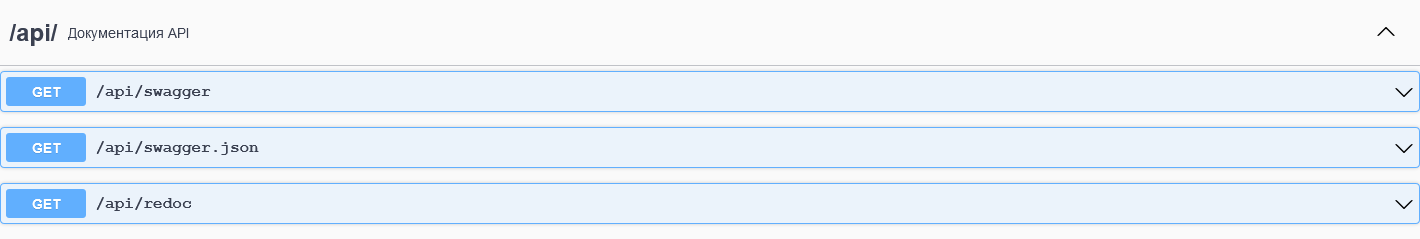
\includegraphics[width=18cm]
  {images/api.png}

  \caption{Документация}
  \label{fig:SwaggerApi}
\end{figure}

\begin{figure}[!p]
  \centering

  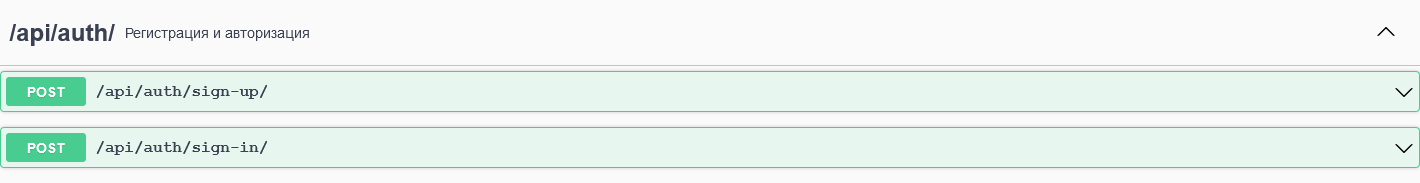
\includegraphics[width=18cm]
  {images/api-auth.png}

  \caption{Регистрация и авторизация}
  \label{fig:SwaggerApiAuth}
\end{figure}

\begin{figure}[!p]
  \centering

  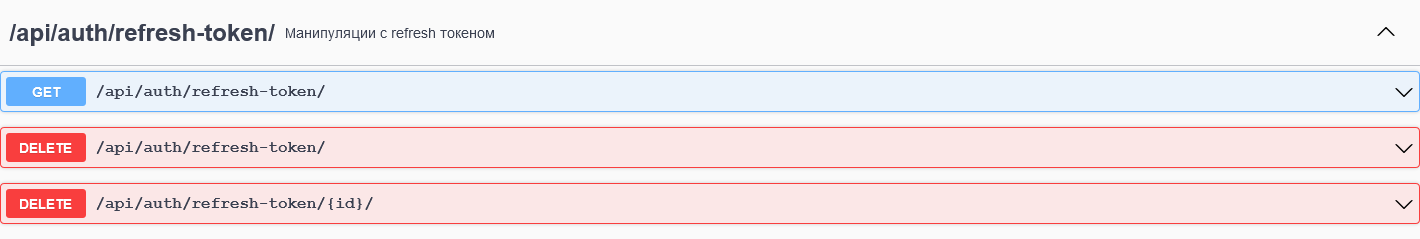
\includegraphics[width=18cm]
  {images/api-auth-refresh-token.png}

  \caption{Манипуляции с refresh токеном}
  \label{fig:SwaggerApiAuthRefreshToken}
\end{figure}

\begin{figure}[!p]
  \centering

  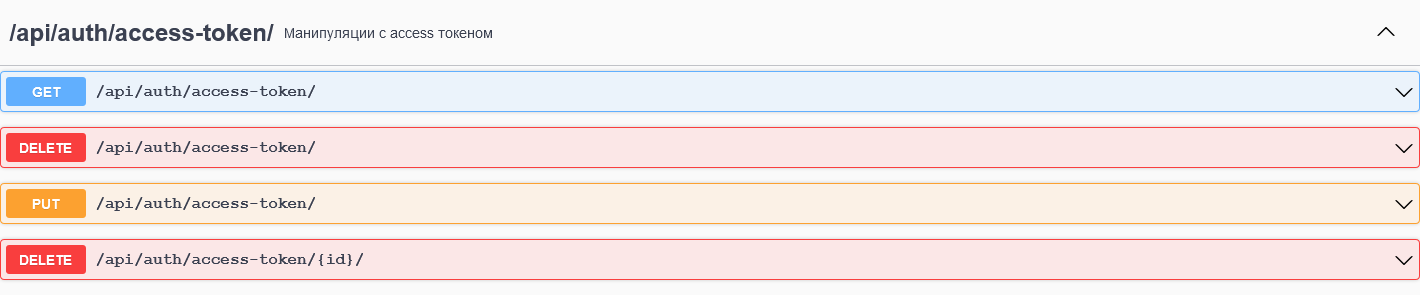
\includegraphics[width=18cm]
  {images/api-auth-access-token.png}

  \caption{Манипуляции с access токеном}
  \label{fig:SwaggerApiAuthAccessToken}
\end{figure}

\begin{figure}[!p]
  \centering

  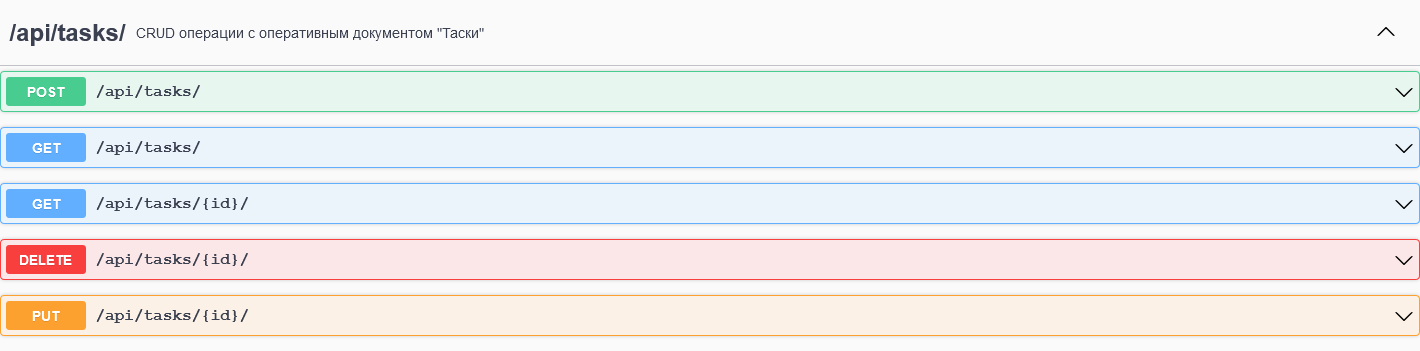
\includegraphics[width=18cm]
  {images/api-tasks.png}

  \caption{Манипуляции с мероприятиями}
  \label{fig:SwaggerApiTasks}
\end{figure}
% = = = = = = = = = = = = = = = =


% = = = = = = = = = = = = = = = =
\newpage
\subsection{Диаграмма последовательностей (Sequence Diagram)}

Диаграмма последовательностей для авторизация изображена на рис.~\ref{fig:SequenceDiagramSignIn}

\begin{figure}[!h]
  \centering

  \includegraphics[width=18cm]
  {../design/UML/export/SequenceDiagram-SignIn-Page-1.pdf}

  \caption{Диаграмма последовательностей для авторизация}
  \label{fig:SequenceDiagramSignIn}
\end{figure}

Диаграмма последовательностей для получения массива мероприятий изображена на рис.~\ref{fig:SequenceDiagramTasks}

\begin{figure}[!h]
  \centering

  \includegraphics[width=18cm]
  {../design/UML/export/SequenceDiagram-Tasks-Page-1.pdf}

  \caption{Диаграмма последовательностей для получения массива мероприятий}
  \label{fig:SequenceDiagramTasks}
\end{figure}
% = = = = = = = = = = = = = = = =


% = = = = = = = = = = = = = = = =
\newpage
\subsection{Диаграмма видов деятельности (Activity Diagram)}

Диаграмма видов деятельности для авторизации изображена на рис.~\ref{fig:ActivityDiagramSignIn}.

\begin{figure}[!h]
  \centering

  \includegraphics[width=18cm]
  {../design/UML/export/ActivityDiagram-SignIn-Page-1.pdf}

  \caption{Диаграмма видов деятельности для авторизации}
  \label{fig:ActivityDiagramSignIn}
\end{figure}

\newpage
Диаграмма видов деятельности для получения массива мероприятий изображена на рис.~\ref{fig:ActivityDiagramTasks}.

\begin{figure}[!h]
  \centering

  \includegraphics[width=18cm]
  {../design/UML/export/ActivityDiagram-Tasks-Page-1.pdf}

  \caption{Диаграмма видов деятельности для получения массива мероприятий}
  \label{fig:ActivityDiagramTasks}
\end{figure}
% = = = = = = = = = = = = = = = =


% = = = = = = = = = = = = = = = =
\newpage
\subsection{Графический интерфейс приложения (UI/UX)}

Макет страницы мероприятий на год на рисунках~\ref{fig:UxYearPage},~\ref{fig:UiYearPage}.

\begin{figure}[!h]
  \centering
  \begin{minipage}{0.32\textwidth}
    \centering
    \includegraphics[width=0.99\textwidth]
    {../design/UX/export/YearPage-Page-1.pdf}
    \caption{UX мероприятий на год}
    \label{fig:UxYearPage}
  \end{minipage}
  \begin{minipage}{0.66\textwidth}
    \centering
    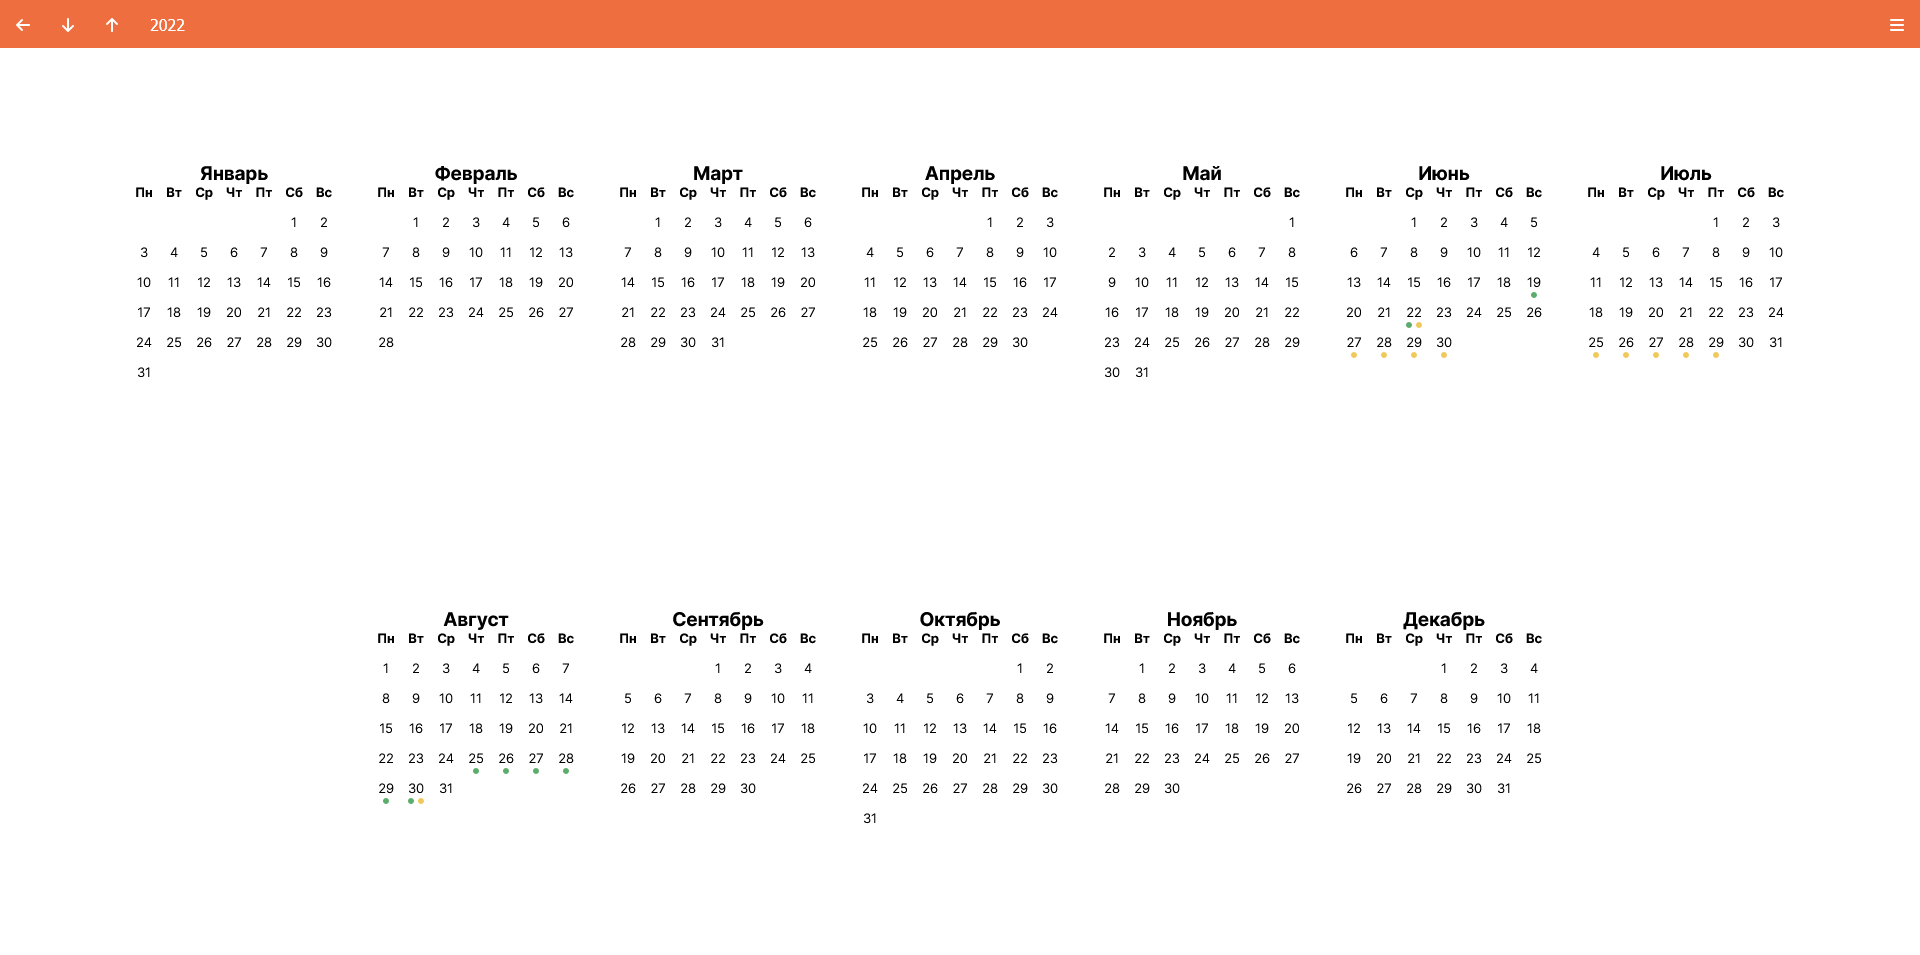
\includegraphics[width=0.99\textwidth]
    {images/screenshots/YearPage.png}
    \caption{UI мероприятий на год}
    \label{fig:UiYearPage}
  \end{minipage}
\end{figure}

Макет страницы мероприятий на месяц на рисунках~\ref{fig:UxMonthPage},~\ref{fig:UiMonthPage}.

\begin{figure}[!h]
  \centering
  \begin{minipage}{0.32\textwidth}
    \centering
    \includegraphics[width=0.99\textwidth]
    {../design/UX/export/MonthPage-Page-1.pdf}
    \caption{UX мероприятий на месяц}
    \label{fig:UxMonthPage}
  \end{minipage}
  \begin{minipage}{0.66\textwidth}
    \centering
    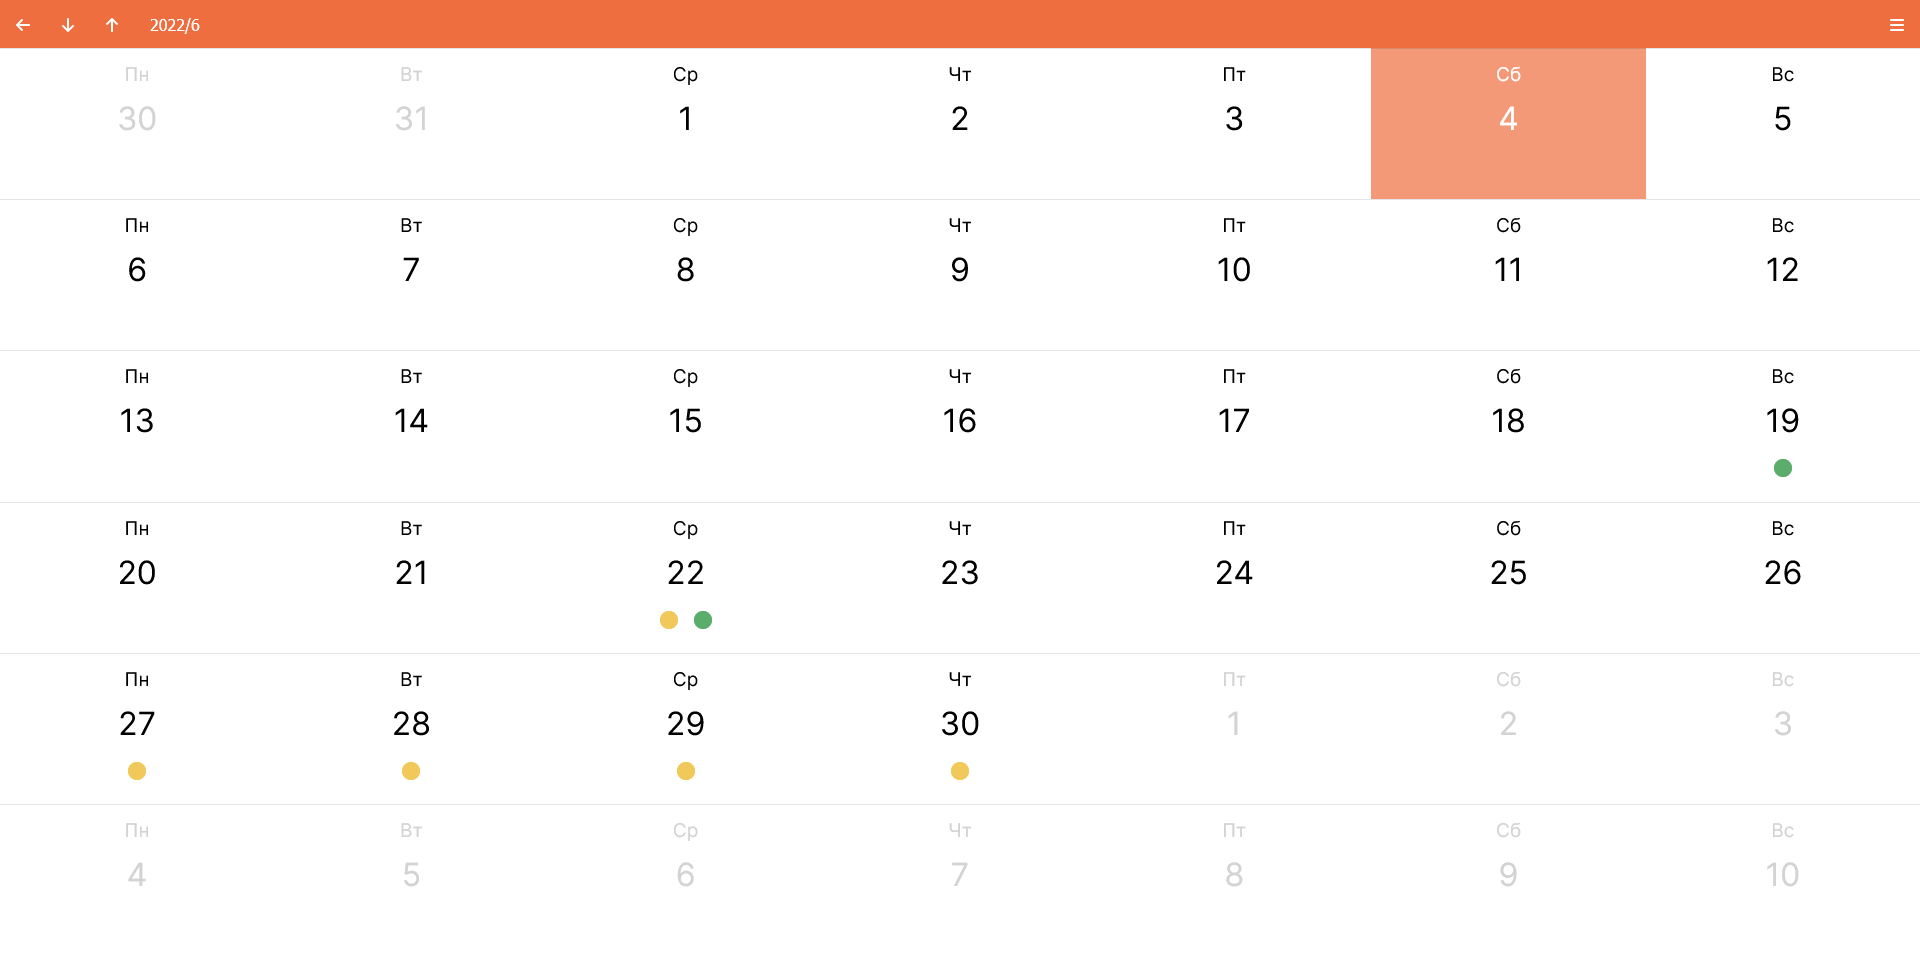
\includegraphics[width=0.99\textwidth]
    {images/screenshots/MonthPage.png}
    \caption{UI мероприятий на месяц}
    \label{fig:UiMonthPage}
  \end{minipage}
\end{figure}

Макет страницы мероприятий на день на рисунках~\ref{fig:UxDatePage},~\ref{fig:UiDatePage}.

\begin{figure}[!h]
  \centering
  \begin{minipage}{0.32\textwidth}
    \centering
    \includegraphics[width=0.99\textwidth]
    {../design/UX/export/DatePage-Page-1.pdf}
    \caption{UX мероприятий на день}
    \label{fig:UxDatePage}
  \end{minipage}
  \begin{minipage}{0.66\textwidth}
    \centering
    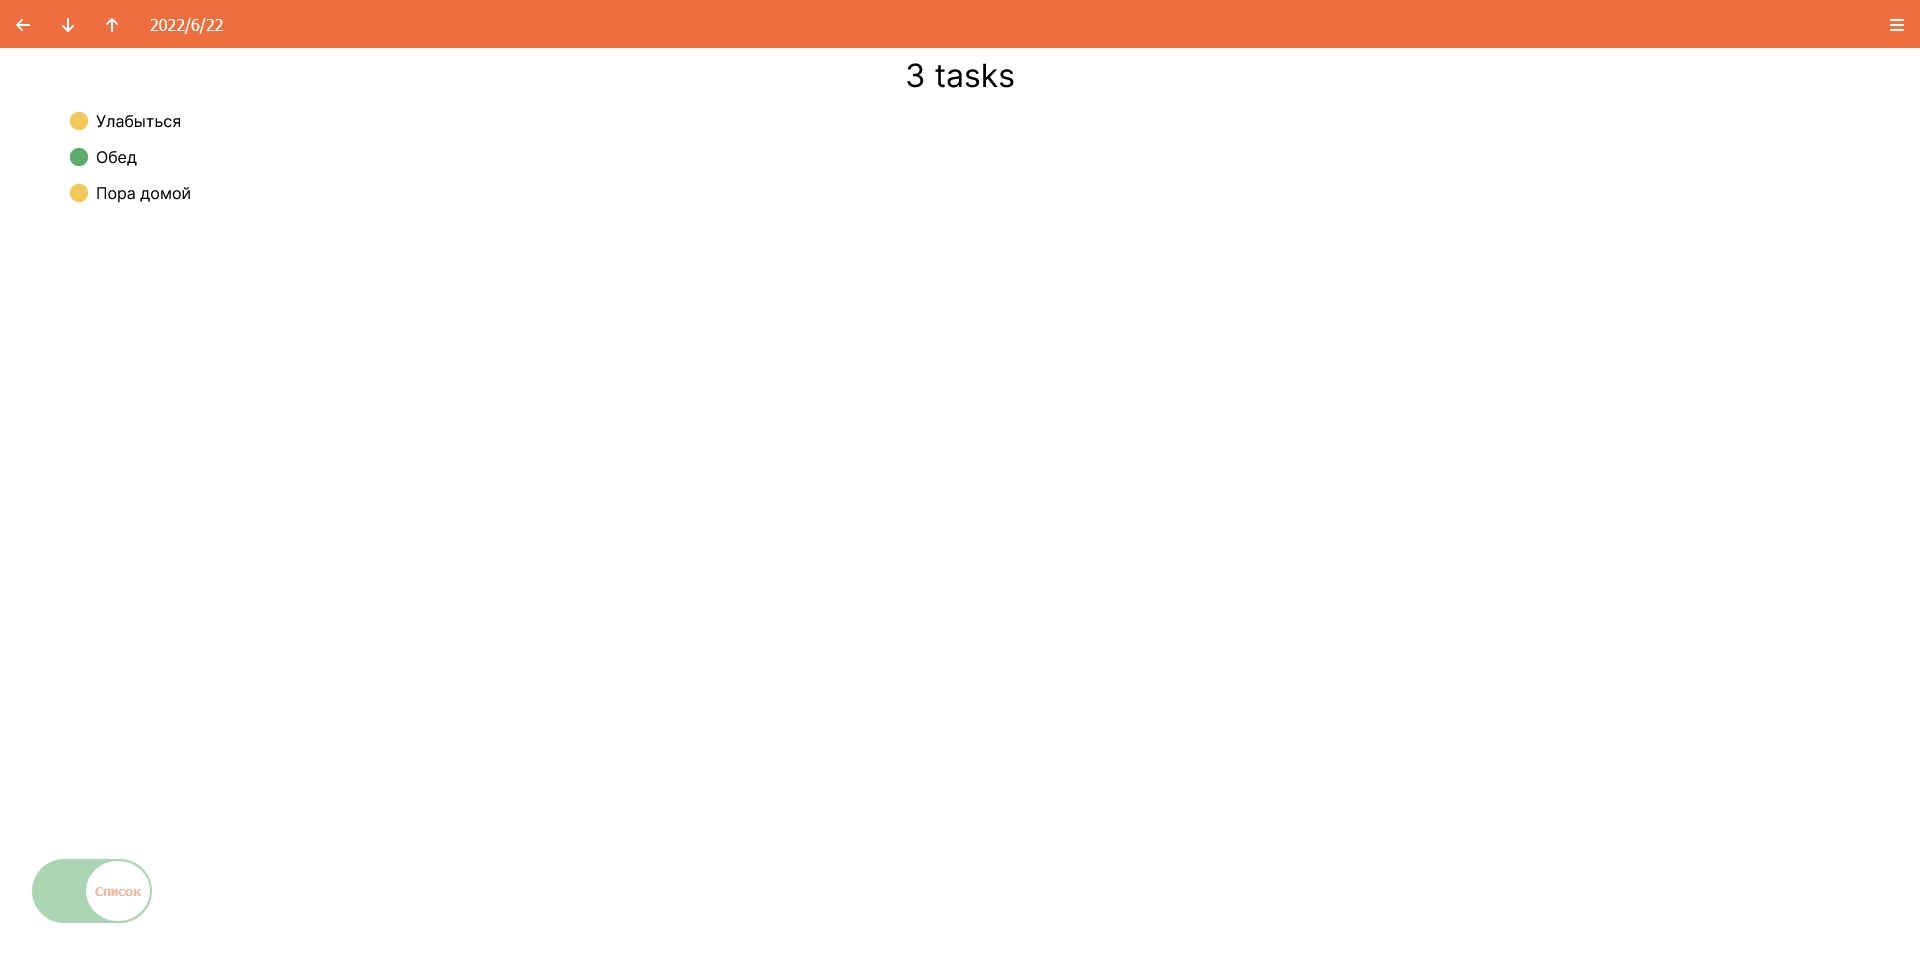
\includegraphics[width=0.99\textwidth]
    {images/screenshots/DatePage.png}
    \caption{UI мероприятий на день}
    \label{fig:UiDatePage}
  \end{minipage}
\end{figure}

Макет страницы мероприятий по часам на рисунках~\ref{fig:UxDatePage},~\ref{fig:UiDatePage}.

\begin{figure}[!h]
  \centering
  \begin{minipage}{0.32\textwidth}
    \centering
    \includegraphics[width=0.99\textwidth]
    {../design/UX/export/HourPage-Page-1.pdf}
    \caption{UX мероприятий по часам}
    \label{fig:UxDatePage}
  \end{minipage}
  \begin{minipage}{0.66\textwidth}
    \centering
    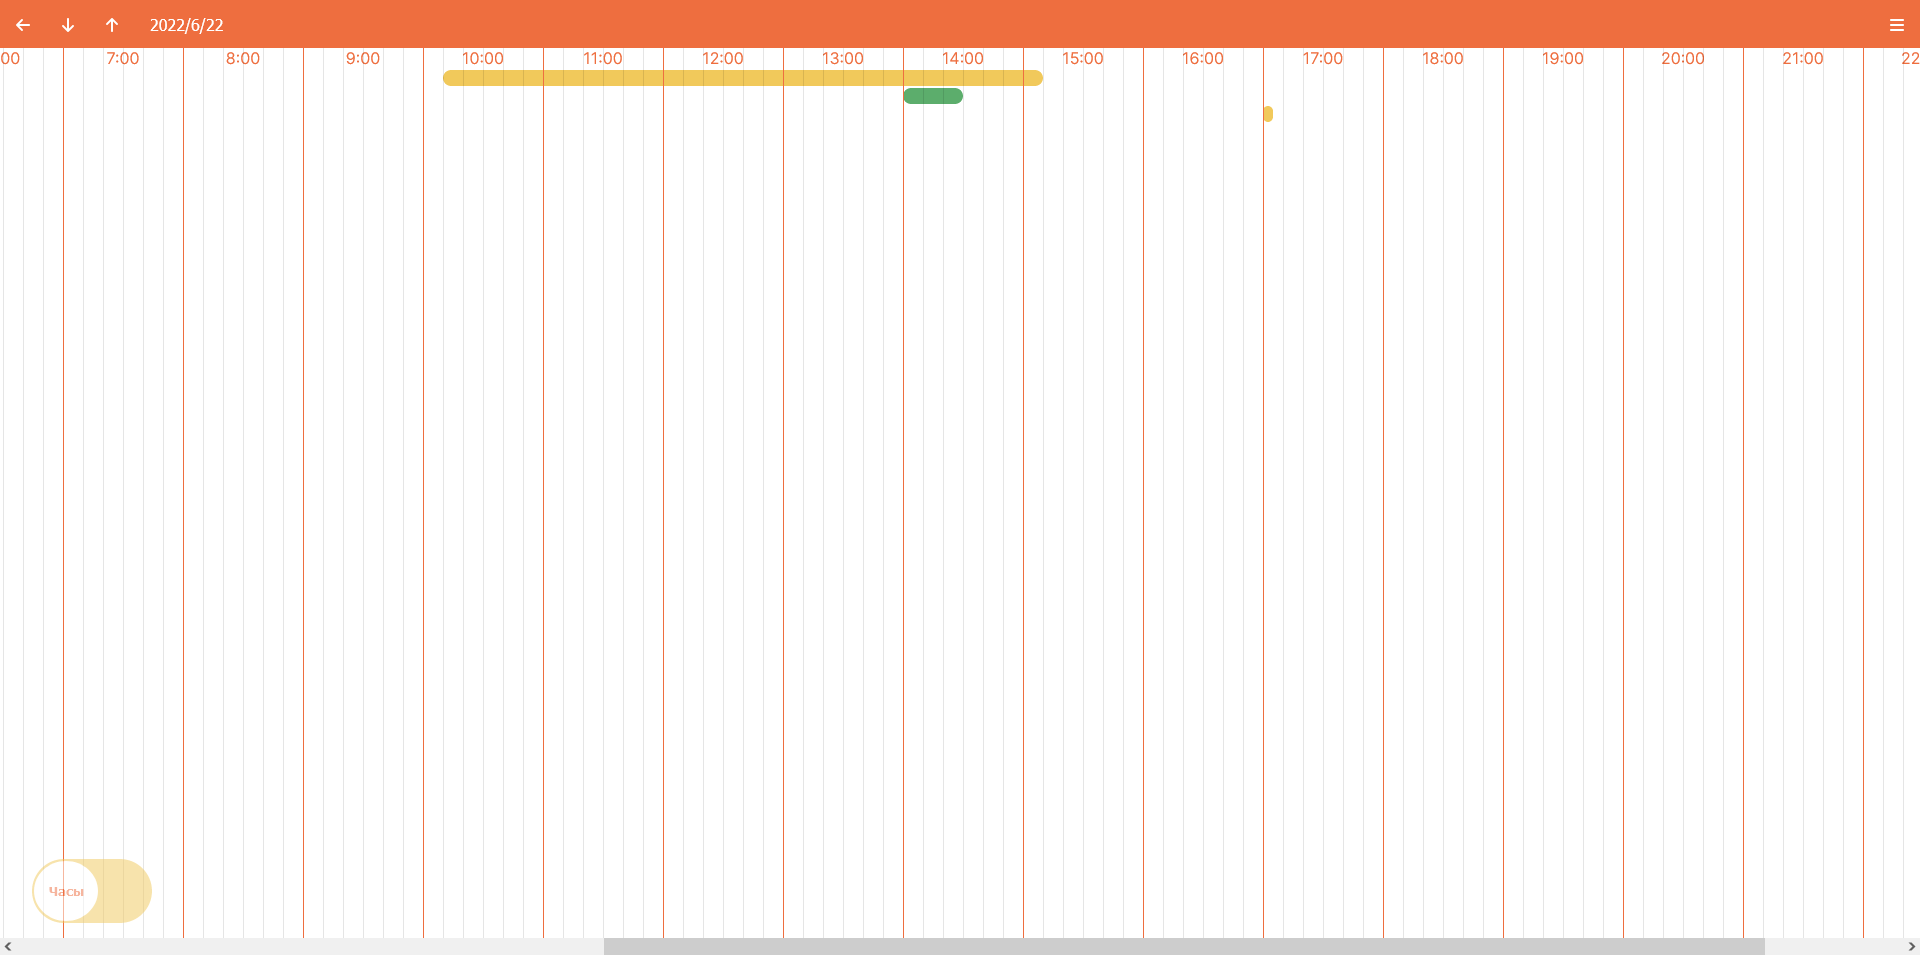
\includegraphics[width=0.99\textwidth]
    {images/screenshots/HourPage.png}
    \caption{UI мероприятий по часам}
    \label{fig:UiDatePage}
  \end{minipage}
\end{figure}

Макет создания мероприятия на рисунке~\ref{fig:UiDatePage}.

\begin{figure}[!h]
  \centering
  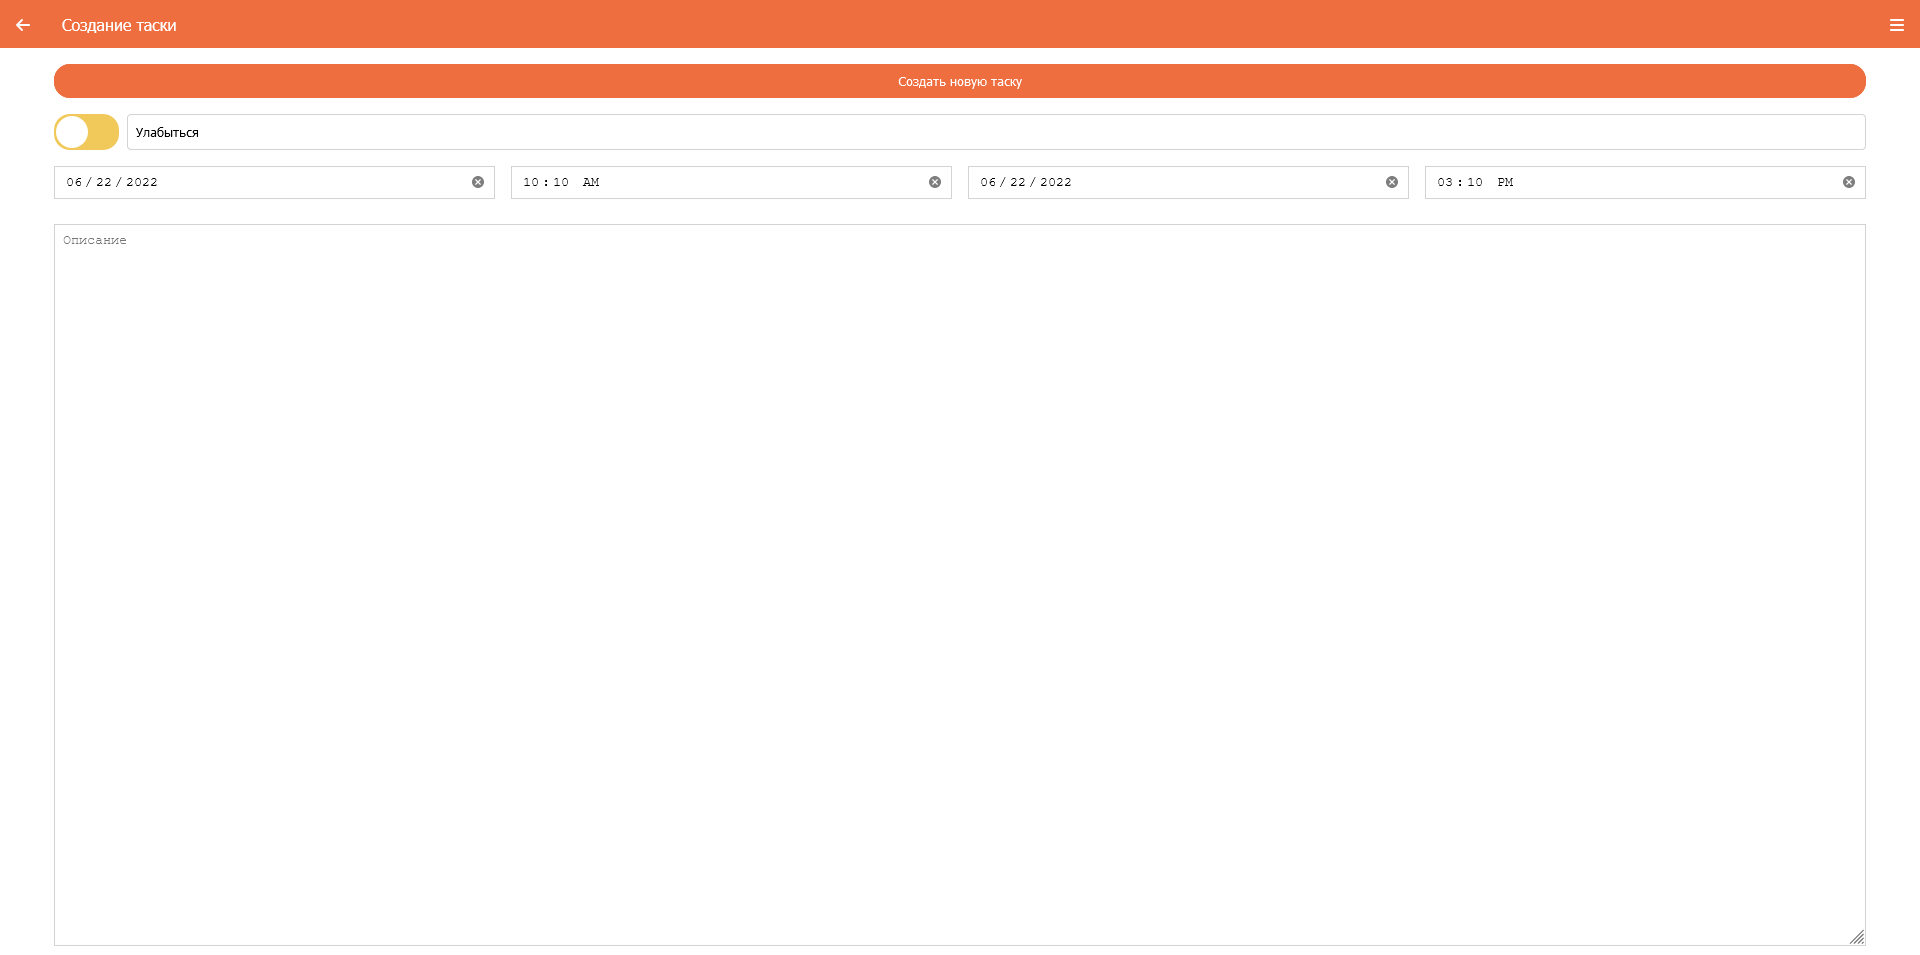
\includegraphics[width=16cm]
  {images/screenshots/TaskPage.png}
  \caption{UI создания задачи}
  \label{fig:UiDatePage}
\end{figure}

% = = = = = = = = = = = = = = = =
